%==============================================================================================
% CHAPTER BINARY RE-WRITER AND VERIFIER
%==============================================================================================
\section{Binary Re-Writer and Verifier}
\label{sec:writeverify}
%
As described in Section~\ref{sec:mmapchecker}, memory protection is
established through run-time checks. 
%
In this section, we discuss a system that introduces these checks by
rewriting the binaries produced by a cross-compiler toolchain.
%
The routines that implement the checks are located in the trusted
domain.
%
The rewriter introduces calls and jumps that invoke the runtime
checks from the sandboxed binary.
%
A verifier inspects the sandboxed binary to ensure that sufficient
checks have been introduced to prevent any possible protection
violation.
%
The verifier and rewriter are completely independent, and
%
the node that executes a sandboxed binary needs to trust only the
verifier.
%
The verifier could be a desktop application that, for example,
cryptographically signed binaries, or a trusted component running on the
sensor node.
%
%% If the verifier is a desktop application, the verified binary needs to
%% be cryptographically signed before being injected into the network.
%
%% The node needs to verify the cryptographic signature of a binary
%% before it is admitted for execution.
%
Our verifier is a trusted component running on every sensor
node that verifies sandboxed binaries locally prior to admitting them
for execution.
%
Sandboxed binaries can be seen as an example of proof-carrying code
(PCC)~\cite{necula96pcc}, even though they do not include any logical
proofs.
%
An attractive feature of this architecture is that sensor nodes do not
need to trust any external component.
%
We discuss the tradeoffs involved in the design of the verifier in
Section~\ref{sec:verifydesignspace}.
%
%==============================================================================
% INLINE CHECKS
%==============================================================================
\subsection{Sandboxed Operations}
%
Five types of operations are protected by the sandboxer.
%
\begin{enumerate}
%
\item{All forms of store instructions are sandboxed by a call to the
memory map checker.}
%
\item{All function call entry points are instrumented with calls to
the function entry stub, which uses the safe stack.}
%
\item{All return instructions are redirected to the function exit stub.}
%
\item{All computed calls are redirected to a stub that checks if
the destination is in the jump table.} 
%
\item{The beginning of all the basic blocks are marked by a special
\texttt{NOP} symbol.}
%
\end{enumerate}

An example of the sequence of instructions introduced by the rewriter for
the AVR architecture is shown in Figure~\ref{fig:inlinechecks}.
%
The sequence is re-entrant; it can be preempted by interrupts.
%
%Push and pop instructions used in sandboxing store instructions can be removed by using dedicated registers.
%
%However, the AVR-GCC register allocator does not support using dedicated registers.
%
The rewriter performs a basic block analysis of the binary and preserves
the program's original control flow by updating static jump, call, and
branch targets.

\begin{figure}[htbp]
   \centering
   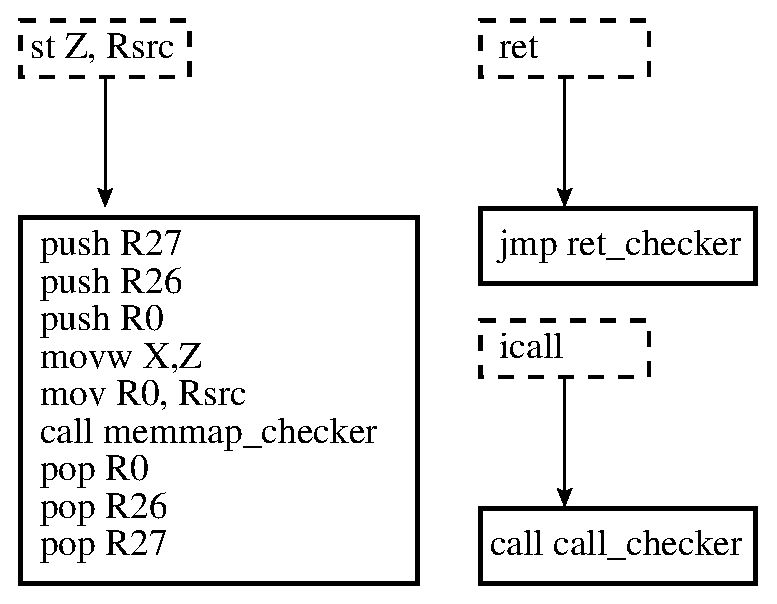
\includegraphics[height=1.75in, keepaspectratio=true]{figures/rewriter.eps} 
   \caption{Inline Checks}
   \label{fig:inlinechecks}
\end{figure}
%

The rewriter reads ELF object files.
%
It uses symbol table information to
distinguish binary data representing code and constants.
%
Upon sandboxing, the rewriter outputs a new ELF object file.
%
The symbol table and the relocation records in the output ELF file are
suitably modified to reflect their updated positions within the
sandboxed code.
%
Since linkers such as \texttt{avr-ld} link object files in ELF format,
%
the binary rewriter can be used to sandbox only portions
of the complete binary.
%
For example, only the device drivers in the final image of an
operating system can be sandboxed before installing them on a sensor
node.
%

%
%
%==============================================================================
% VERIFIER
%==============================================================================
\subsection{Verifier}
%
The verifier is a very simple program that maintains no state.
%
In Harbor, all potentially unsafe operations, such as store to
memory, returns, and computed calls, are performed within the
run-time checkers.
%
Therefore, the verifier performs a single pass over the entire
instruction sequence and raises an exception if it encounters
any of the potentially unsafe operations. 
%such as stores, returns and computed call/jump instructions.
%
It checks all static jump, call, and branch targets to ensure that
they are within domain boundaries.
%
It also ensures that these targets point to valid instructions.
%
This check is necessary because AVR ISA has multi-word instructions.
%
If control flow jumped into the middle of a multi-word instruction,
run-time checks might be circumvented.
%
Therefore, the rewriter marks the beginning of basic blocks with a special
\texttt{NOP} symbol.
%
The verifier checks that all static jump, call, and branch targets
point to a \texttt{NOP}, and checks that the \texttt{NOP} symbol never
appears in the middle of a multi-word instruction.
%
%% The basic blocks are marked by a special \texttt{NOP} symbol; which is
%% checked to ensure to appear elsewhere in the 
%% %
%% Therefore, control flow can jump into the middle of a multi-word
%% instruction and circumvent the run-time checks.
% 
%Our current implementation of the verifier does not detect this.}
%
Function entry points (determined from call instruction targets) are
checked to ensure that they store the return addresses on the safe stack.
%
Finally, the verifier does not permit store instructions that write to
program memory.
%
The verifier calls an exception handler if any of these properties are violated.
%
Its total line count is only 211 lines.
%
%----------------------------------------------------------------
\subsection{Verifier Design Tradeoffs}
\label{sec:verifydesignspace}
The Harbor design also allows trading off execution overhead, and code size
increase, against the complexity of the verifier.
%
Performance and code size increase are directly proportional to the
number of operations that are sandboxed.
%
The current implementation sandboxes \textit{all} unsafe operations.
%
This severely penalizes performance and code size but reduces the
complexity of the verifier, which requires only a single pass over the
entire binary and maintains no additional state.
%
Static analysis on the binary can reduce the number of operations
sandboxed by adding single checks that safely protect a series of
potentially unsafe operations.
%
However, the safety of such a check is harder to verify using a simple
verifier.
%A single check can be used to protect a series of potentially unsafe operations.
%
%A complex verifier can permit direct execution of potentially unsafe operations (such as stores) that have been protected by earlier checks.
%
An interesting area of future work is to explore this design space to
develop a rewriter--verifier combination that consumes limited
resources but improve performance, and reduces code size, of sandboxed
binaries.
